%************************************************
\chapter{Combined Alternative Positioning and Signalling System}\label{ch:COMPASS}
%************************************************
\section{Introduction}
In the financial year 2015/16 Network Rail spent £106,008,691.22 \footnote{This information is made available by Network Rail at \url{https://www.networkrail.co.uk/who-we-are/transparency-and-ethics/transparency/datasets/}. The relevant data is headed \say{Payments for disruption on the railway made under schedule 8} and further data is available for schedule 4, planned disruptions.} compensating operating companies for unplanned delays. Every week many tens of thousands of delay minutes accrue on the railway, and of these many thousands are attributed to signalling failures. The delay caused to passengers as a result of such failures degrades customer experience and contributes to negative public perceptions of the railway. The Combined Positioning Alternative Signalling System,(COMPASS), is a system to provide a degraded mode signalling system with the primary objective of reducing the impacts associated with failures of the main signalling system. Fringe benefits of such a system also include improved vehicle positioning relative to the existing track circuit based system, leading to improved passenger information and the potential for use as a low cost primary signalling system on lightly used lines. 

The COMPASS project was carried out in conjunction with industrial partners, and thus it was important that the end result was a demonstrator that could become a commercially viable product. This enabled the investigation of those questions pertaining to the available skills within the industry, those related to the deployment of ontology based architectures on a large scale alongside providing a means of verifying the work done in \autoref{ch:middleware}.

\subsection{Commercial Partners}
The university of Birmingham carried the project in conjunction with Siemens (Westinghouse) and Park Signalling Ltd. All ontology and data integration based work was undertaken by the author, whilst the other partners provided all other subsystems and made engineering support available for integrating them  

\subsection{The commercial case for degraded mode signalling}
The involvement in this project of commercial partners demands that it have a business case, in this case the project was completed in response to a request from Network Rail in conjunction with the railway safety and standards board and Future Railway. 

According to Network Rail historic delay attribution data  \citep{NetworkRailInfrastructureLtd2017}, signal failures are responsible for a significant proportion of the delays on the UK rail network. Delays from a single type of signalling failure (track circuit failures) contributed 103260 minutes (over 71 days) of aggregated delays over a single 28 day reporting period, and these represent the largest delay for which the infrastructure manager is responsible. The industry is keen to explore potential solutions to issues caused by signalling delays. Network Rail, upon whom the costs fall, are particularly keen, as stated in \citet{MagazineRailTechnology2015} 
\begin{quote}
    [Network Rail] believe the COMPASS solution can reduce delays by improving the current signalling system’s ability to recover from system failures more rapidly, as well as providing enhanced resilience to the network for the future. 
\end{quote}

\subsection{Objectives}
In the tender request the customer (Network Rail) gives the purpose of the system as: ``to automate the manual processes involved in Temporary Block Working''. Temporary block working is the current fall-back procedure whereby trains are allowed to pass through sections of track where the signalling has failed. Several consortia are creating products in response to this tender and it is possible that more than one will be selected. In the UK rail domain the Infrastructure owner merely specifies systems, they do not design or build systems themselves, however they will evaluate the system in accordance with the tender document. To add complexity in this case the desired specification requested by the infrastructure manager changed over the lifetime of the project, as did the personnel allocated to it. This is a common challenge in real projects and thus representative of projects within the UK rail domain. Notably the amount of automation expected was reduced and the requirements altered such that there must always be a man in the loop. Furthermore it was clarified that the system would at no time be an \say{Alternative Signalling System}, rather it was to provide \say{Degraded Mode Working} and would never be used outside of those circumstances. 

The COMPASS demonstrator aims to show how ontology can form the core of a fall-back signalling system, reducing the impact of signalling system failure, keeping trains moving even when the main system has failed. The proposed solution is agnostic to the failed signalling system - either a traditional national signalling system employing a fixed block system or a modern moving block system.

The demonstration scenario assumed new equipment could be placed in two physical locations: In Cab, and in the Rail Operating Centre (here on ROC - effectively a control centre or modern signal box). It should be noted that cost is also important, this system cannot cost as much as a main signalling system, as such certain compromises are required. Guidance from Network Rail suggests that points should not be remotely controlled, rather the lie of the points (also known as switches or turnouts) should be detected and trains only routed where that permits. This reduces the safety criticality of the software and thus the level of (expensive) certification required. In particular the infrastructure operator wished to avoid the need for SIL level 4 certification, as such it was also requested by Network Rail that the system not issue trains authority to move without manual intervention. It is expected that improved knowledge of train location will also make possible improved passenger information.

\subsection{Client Requirements}
\label{sec:client}
The requirements from the client were set out in a tender documents \citep{NetworkRailInfrastructureLtd2015} and modified verbally, they may be summarised as:
\begin{itemize}
    \item The replacement of temporary block working with a more efficient solution. Originally this was the automation of temporary block working, however in light of guidance from the infrastructure manager there will still be a manual element;
    \item The system shall be deployed in a limited number of predetermined areas, were signal failures risk the greatest impact. This also differs from the original specification, which required scalability up to providing a national train position database. The area need not be a plain line, but can and likely will have multiple entrance and exit signals. The area can be bi or uni directional.
    \item The accuracy of train location data and hence arrival times estimation should be better than is available from the existing track circuit based systems;
    \item \say{System shall be separate from the existing signalling system};
    \item Be resilient to cyber attack, physical vandalism and deliberate sabotage;
    \item \say{maintain, in memory, train location to a given time stamp for reference purposes} ;
    \item Ease of adding other datasources when they become available would be an advantage;
    \item \say{adopt a multi-layered solution for train location.} That is take train position information from multiple sources. 
\end{itemize}

In order as to achieve the above objectives, in particular, the adoption of a multi-layer train location solution and the improved location accuracy it is necessary to bring together data from multiple sources. Use of an ontology architecture would minimise the development effort required to accomplish this.

\section{System design and specification}
In response to the requirements set-out in \autoref{sec:client} and in conjunction with industrial partners, the demonstration scenarios described in \autoref{sec:Scenarios} were designed. These scenarios made it possible to demonstrate that the techniques selected will be capable of meeting the client's specification and produced a system which, if the client chooses to proceed, can be commercialised. 

The system is referred to by the commercial partners as the \say{Secure Train Information Recovery} system or STiR and that name is used throughout this document.
\subsection{Demonstrated scenarios}
\label{sec:Scenarios}
Two demonstrations were performed, in response to two different operational scenarios: The first demonstrates normal operation; the ontology with supporting tools connects to and process data-feeds from the UK infrastructure owner, Network Rail; this could include providing improved customer information. The second demonstration focused on the degraded mode operation itself and showed how vehicles could transition to COMPASS signalling and pass through a failed area of control. More details are given in \autoref{sec:demotwo}.

\subsubsection[Normal Operation]{Normal Operation - Quiescent State \\ First Scenario}
In the first scenario the railway is assumed to be operating normally, with the system in what is referred to as a ``Quiescent State''. In COMPASS this is used to demonstrate the system  monitoring the locations of services already running over the network, ready for use as the \say{base state} when a failure occurs. The train location data used in this scenario came from the Network Rail open data feeds, which were used in conjunction with a static map of the network, provided by the industrial partner. These two diverse data sources provide good examples of typical industry data sources, that may need integration in a functioning industry wide system. 

In normal operation the demonstrator tracks the locations of all the trains in the network, allowing the provision of better customer information as well as maintaining a model of the running system in readiness for degraded mode operation. This demonstrates that should a signalling fault occur the system would be able to respond appropriately. Tracking of locations is illustrated by displaying those positions on a map, annotated with the headcodes of the trains being tracked. A proposed extension to this scenario calls for the display of metadata for the train - projected arrival time for example - along with the headcode. The use of ontology in this project also makes easier displaying such things as live updated possible connections, in light of the arrival time. 

The quiescent state demonstrator monitors vehicle movements across the entire British rail network, and as a result provides solid evidence of the ability of ontology based systems to scale to the data volumes and rates needed in a nationwide industry deployment.

\subsubsection[Degraded Mode]{Degraded Mode \\ Second Scenario}
Degraded mode occurs when the underlying signalling system is not operating as intended, regardless of reason, and signaller chooses to use the COMPASS system to manage the train through the area, known within this project as the \say{area of interest}. It is expected, though not required, that the area will be relatively small and when the end of the area is reached the train returns to the control of the primary signalling system. 


\subsection{System Architecture}
A system was designed to meet the client requirements, which was capable of performing the demonstrations outlined in \autoref{sec:Scenarios}. This required sub-systems from multiple suppliers and which would, in implementation, be split between the signalling control centre, known in the UK as a \say{Rail Operating Centre} and the cab of every train fitted with the technology. For demonstration purposes all systems were present in the same room and physically connected; radio telecommunications being beyond the scope of the demonstrations. The demonstration system adopted the architecture set out in \autoref{fig:fullsys}. 

\begin{figure}[H]
\myfloatalign
{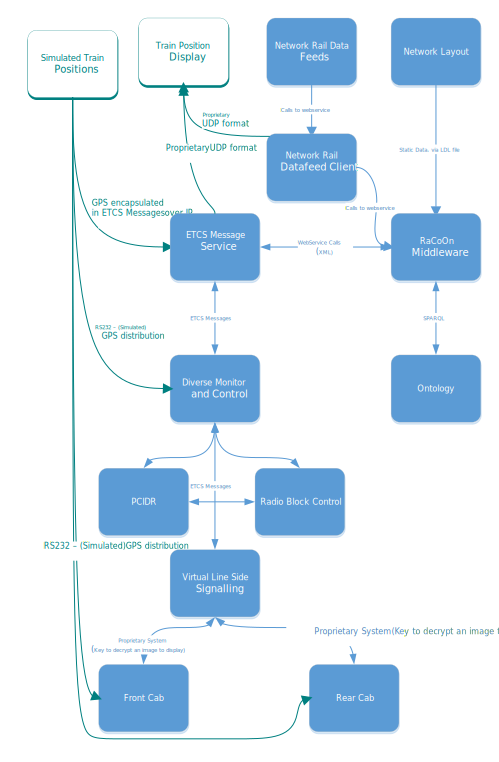
\includegraphics[max height=\textheight,max width=\linewidth]{gfx/FullSystem}} 
\caption{Full System Dataflows}
\label{fig:fullsys}
\end{figure}

The purpose of each sub-system is described in \autoref{sec:demoTwoOrg}. 

\subsubsection{Degraded Mode Demonstrator Organization}
\label{sec:demoTwoOrg}
The following elements are housed in the control centre:

\begin{description}
    \item[VLS Centre Comms] Virtual Line-side Signalling, which handles communications between the in cab elements and the control centre elements. This is a pre-existing commercial product modified for this project.
    \item[DMC - Diverse Monitor and Control] This component acts a central control block bringing all the other subsystems.
    \item[RBC - Radio Block Control] This is a standard part of a moving block signalling system.  It is a pre-existing commercial product which handles safety critical aspects of the system.
    \item[PCIDR]  \textit{Track based Point Control Inhibit, and Detection Repeat (PCIDR) and Control} \\
    This `isolates' the points (switches). Whilst the system is in operation the points do not move. The current position of the points is detected and fed back to the rest of the system, which will only signal trains to pass in directions allowed by the points.
    \item[STiR Interlocking] This is a simplified version of a conventional signal interlocking, since the points are isolated.
    \item[RaCoOn] The Railway core ontologies. This integrates data from a number of different external and internal sources, alerting the other components when a train is approaching. This in turn comprises a number of sub-systems:
    \begin{itemize}
        \item The ETC Message service; This receives ETCS messages and triggers appropriate changes to the ontology;
        \item The RaCoOn Middleware, as discussed in \autoref{ch:middleware} it acts as a buffer between the others systems and the datastores;
        \item The datastores;
        \item A system to display train locations on a map. In this case an existing rail simulator, BRaVE which discussed further by \citet{Wen2015}.
    \end{itemize}

\end{description}

The data flows between these elements are illustrated in \autoref{fig:dataflow}. In order as to display instructions to the train driver (the system does not employ automatic train control at this point) a further in cab element is required. There are additional components used only for demonstration purposes, and would not have been included in the finished system.

\begin{figure}[H]
\myfloatalign
{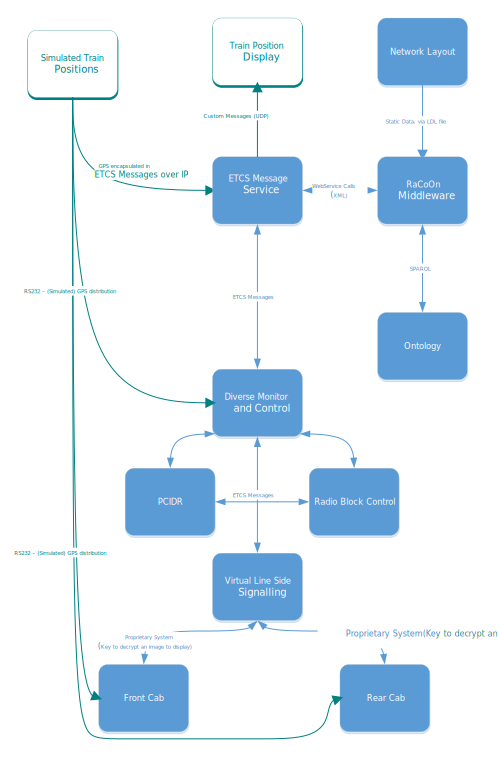
\includegraphics[max height=\textheight,max width=\linewidth]{gfx/Dataflow-StirDemoActive}} 
\caption{Demonstrator Two Dataflows. Note that links in green are demonstration only - not part of the final solution}
\label{fig:dataflow}
\end{figure}

As can be seen from \autoref{fig:dataflow} links between sub-systems, in particular those from different suppliers, use ETCS messages for communication. ETCS (discussed in \autoref{sec:etcs}) uses a standardised set of messages for communication with the train, and these messages are employed here between sub-systems. This was chosen for a number of reasons; firstly the industrial partners in this project had pre-existing expertise with this standard. Secondly the standard can easily be implemented over an Ethernet link, simplifying connection and lastly some sub-systems could only communicate in this manor. 

In order as to demonstrate the system it was necessary to use a rail simulator to recreate the effect of the train being in motion. The simulator generated coordinates representing the position of the front of the simulated train. These were sent to the in-cab signalling equipment in the same format as would have been used were the data coming from a real GPS receiver mounted on a train\footnote{A NMEA string delivered over a serial bus (RS232)}. The same position data was then sent to RaCoOn, to simulate the train sending position data. 


\section{Data Sources}

A number of specific data resources would be needed to support the demonstrators outlined in \autoref{sec:Scenarios}. These are detailed in the following sections and illustrated in \autoref{fig:AllSources}:

\begin{figure}[h]
\myfloatalign
{\includegraphics[width=\linewidth]{gfx/DataflowStirAllOptionsDemo}} 
\caption{All Possible Data Sources for integration}
\label{fig:AllSources}
\end{figure}


\subsubsection{Schedule Data}
For this project schedule data was obtained in the format of CIF files. This is a dense data format, holding weekly advance schedules.

Schedule data is comparatively coarse, primarily listing station calling times, alongside some supplementary information regarding the type of rolling stock used. In this file the trains are identified by headcode, which is unique on the rail network at any one time, however multiple trains are assigned the same headcode at different times. A further unique identifier is therefore supplied, which can be linked to other data feeds, but not directly the train describer feed, which uses only the headcode. This datasource is described in more depth in \autoref{sec:datatoimport}.

This is parsed using the tool described in \autoref{ch:cifparser}.
   
\subsubsection{Train movement data}
Train movement data, from the Network Rail webservices in particular the train describer feed. This feed supplies messages when a train steps from one signalling ``berth'' to the next.

Data is taken from the train describer feed, which is provided by Network Rail \footnote{available at: \url{stomp:tcp://datafeeds.networkrail.co.uk:61618}}. This feed provides messages from the train describer, which is a part of the signalling system that provides information to the signaller. This demonstrator uses only the ``Berth Step'' messages, which are generated whenever a train moves from one berth to the next. In the context of a signalling system berths are a region of track, protected by a signal, in which a train is located, a further definition may be found in \citet{Woolford2004}. As such the progress of a train across the network can be tracked, if used in conjunction with a map of signalling berths.

For this project it provided one of the key sources of train location data, obtained on a national level, to demonstrate the ability of the system as a whole and ontology in particular to process data on this scale.

\subsubsection{Absolute Position Data}
The absolute position of a rail vehicle, that is its position relative to the surface of the planet can be obtained from a Global Navigation Satellite System (GNSS), based on timing signals from satellites in known geostationary orbits. Positions are normally derived in terms of latitude, longitude and altitude which then needs combining with further data (typically a map) in order as to be meaningful to users. The Global Position System is the oldest and implementation of this and is the system chosen for this project, based on the low cost of compatible hardware. Were this project commercialised a full evaluation of the available options would be required.

Position can be expressed using multiple coordinate systems and projetions. The system chosen depends on the area that needs to be represented and how the data needs to be manipulated. A through review of map projections is well behind the scope of this thesis, however the following projections were used:
\begin{itemize}
    \item WSG84
    \item OSG36
\end{itemize}
WSG84 is the standard coordinate system used with GPS. It covers the entire globe, which it models as a spheroid. OSG36, commonly known as British National Grid is a coordinate system used only within Great Britain. It used only for display purposes in this project, since the available maps for displaying data used this format. 

It is intended that when this project is implemented GPS provides the more accurate data stream, allowing for better customer information and providing a fall-back in the case of failed track circuits, as well as making it possible to run trains closer together.

GPS data was simulated for the demonstrators. The data recreated a feed from a GPS unit fitted to a train cab and as such the data was supplied as a standard NMEA string, wrapped in an ETCS message. Accuracy issues were not considered in this demonstrator, had they been there would have been a need to combine balise pass data, to know which line a train was on, with the GPS data, since GPS accuracy is not always enough to know with certainty which of several parallel lines a train is on. The distribution of GPS data is further discussed and illustrated in: \autoref{sec:demoTwoOrg}.

For this project it was sent wrapped in standard ETCS messages, using packet 44, which is reserved for applications outside of normal ERTMS/ETCS operation.

    \subsubsection{Static network layout}
The static track layout information was provided in LDL format.

The network map is static data loaded once and not changed. This network map was obtained in layout description language (LDL) format. LDL Format is a proprietary standard used internally within Siemens to describe the rail network, including all the infrastructure positioned on the network. The information is stored in a human readable and editable form, though tools to edit and display it exist and were used in this project. LDL files list first the most basic infrastructure, track, which is described as a series of nodes and edges, then the positions of increasing complex elements are overlaid, using a node and offset location system. This ``Node - Edge'' way of modelling the rail network sits well with the ontology, which also represents the network as a series of nodes and edges, though these are not the same as the nodes and edges that constitute the ontology. \citet{Tutcher2015} sets out the rational behind the modelling.

    \subsubsection{Additional datasources}
Beyond the datasources listed above it would also be possible to use the following data sources, though they were not fully implemented in the demonstrators produced:
\begin{description}
    \item [Train Movements Feed] This is another open data feed provided by Network Rail;
    \item [VSTP - Very short term plan] This data feed gives details of trains scheduled at short notice;
    \item [Other signalling systems] In particular direct connection to the train describer system (not via the webservices) was suggested for the final implementation of this project;
    \item [GPS data from the rear of the train] This would make it possible to provide accurate train integrity information, as required if implementing ETCS.     
\end{description}

 \section{Role of Ontology}

In the compass demonstrators the primary role of the ontologies is as the basis for data integration across diverse datasources. There are many data sources for this system and it is one of this project's objectives to show that the project partners could work with data from a multitude of heterogeneous sources, not limited to those included in the initial design. 

Ontology is also used for classification in this project, for example for the classification of nodes, which are classified by sub-type. Nodes can be any of the many types of object located on the track such as: simple nodes, points nodes or signals. Most significantly they can be the signals that mark the start of the area of interest; this information is used to determine when to trigger degraded mode operation.

\section{Demonstrator Implementation}
In order as to provide the demonstrations outlined in \autoref{sec:Scenarios} a system was implemented, consisting of sub-systems from all the industrial partners. In moving to production the simulation would no longer be required whilst certification would be, however, the system is designed such that certification should be obtainable. 

\subsection{Demonstrator One}
\subsubsection{Overview}
 
The first demonstrator, that which sought to show the system under normal operation or within its ``Quiescent stated'', aims to show that using the Network Rail data feeds, it is possible to track the location of multiple trains on the network. Physically this is presented as a geographical map showing the train line on which the capability is being demonstrated with labels showing the current location of running trains. The map is presented in \autoref{fig:DemoOneBrave}. As the train steps to a new berth, so these labels move, with the same granularity as is provided by the signalling system. Running on a physically separate system (though this is not required from a performance perspective) a client written specifically for this task displays the messages in a human readable format, as shown in \autoref{fig:DemoOne}. The ontology holds position data for certain signals on the track in the area on which the system was being demonstrated, these are returned to the map via the tool. Where data is not available the ontology returns nothing and thus no message is sent to display system. In this case display is provided by the centre's own simulator, BRaVE, which was being used solely for display purposes.

\begin{sidewaysfigure}
\myfloatalign
{\includegraphics[width=\paperwidth]{gfx/DemoOneBRAVE}} 
\caption[Realtime Train Position via BRaVE]{Realtime Train Position via BRaVE \citep{Wen2015}}
\label{fig:DemoOneBrave}
\end{sidewaysfigure}

\begin{figure}[h]
\myfloatalign
{\includegraphics[width=\linewidth]{gfx/DemoOneScreenShot}} 
\caption[Demonstrator One]{The first Demonstrator in use}
\label{fig:DemoOne}
\end{figure}


\subsubsection{Model Changes}
This demonstrator made significant use of geographical data, \citet{Tutcher2015} gave a number of suggestions as to how geographic data be handled, in particular it recommended the use of the ``W3C Basic Geo Vocabulary''\footnote{\cite{Lieberman2007}}, alongside the RaCoOn \texttt{u:location} class. This recommendation was followed and geographical locations were encoded using that schema. 

Elements relating only to this project, all of which extended elements from the existing ontology, where placed in an application ontology design specifically for the COMPASS project, shared between both demonstrators. As per the guidelines set out in \autoref{ch:cifparser} this was the lowest level at which it was appropriate to model the concepts and avoided adding unnecessary complexity to those modules shared throughout the domain.

\subsubsection{Advantages of this approach}
The most widely discussed advantage of this approach, that is the use of ontology for data integration as opposed to constructing case by case integrations, is that of ease of adding further data sources without alteration to the existing system. The separation of business logic, which can be moved to the ontology, how one decides where the area of interest is for example in this case, also makes for more maintainable and resilient systems. 

\subsubsection{Implementation}
In the first demonstrator the ontology is used to match signal berths to their physical locations. A SPARQL query shown in \autoref{lst:selectsignallocation} is used with the signal's identifier to retrieve its location. This query is triggered by the arrival of a birth step message from the Network Rail train describer feed then, if found, the resulting latitude and longitude are first converted to British national grid coordinates, before being sent onwards to BRaVE for display. 

\begin{lstlisting}[float=h,language=sparql,frame=tb,caption={SPARQL to select a signal location from its identifier. Note some of the features here are Stardog specific, in particular the passing in of the @sigid parameter},label={lst:selectsignallocation}]
SELECT  ?lat ?long
WHERE {
    ?Signal a <http://purl.org/rail/core/Signal> .
    ?Signal dc:identifier ?ident   .
    FILTER( regex(?ident, @sigid )) .
    ?Signal core:relativePosition ?signalPos .
    ?signalPos u:measurementValue ?offsetVal .
    ?signalPos core:locatedOn ?track  .
    ?savedPos core:locatedOn ?track .
    ?savedPos a geo:Feature .
    ?savedPos wgspos:lat ?lat .
    ?savedPos wgspos:long ?long .   
    ?savedPos core:hasOffsetLocation ?savedOffset .
    ?savedOffset u:measurementValue ?savedOffsetVal .  
    FILTER(?savedOffsetVal = ?offsetVal)
}
\end{lstlisting}

\pagebreak

The data flows within this demonstrator are set out in \autoref{fig:DemoOne-DataFlow}, which shows that much of the system remains inactive in this scenario, as much of the system is dedicated to managing the train through areas of failed signalling.

\begin{figure}[H]
\myfloatalign
{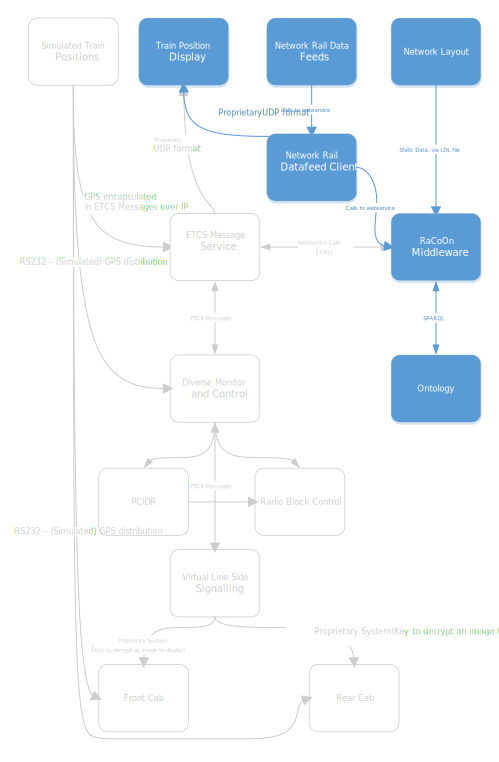
\includegraphics[max height=\textheight,max width=\linewidth]{gfx/Dataflow-StirPassiveDemo}} 
\caption[Demonstrator One Data-flows]{Demonstrator One Data-flows \\ Objects and data-flows shown in grey are connected but inactive}
\label{fig:DemoOne-DataFlow}
\end{figure}


A modular architecture was employed in both demonstrators to allow the reuse of components and to ensure separation between functionally distinct units. The first demonstrator comprised the following modules:

\begin{description}
    \item[MiddlewareConnectivity]
    This was compiled as a DLL and used in both the client to receive Berth Step messages from Network Rail, as used in the first demonstrator, and the tool for receiving ETCS messages used to demonstrate the second scenario. This module provided a range of functions for interacting with the RaCoOn middleware and thus the ontologies and REDIS. For reasons of development time some SPARQL   was embedded in this module rather than being encoded as rules in the ontology. Embedding SPARQL does mean that a certain amount of the process and decision making embedded in the software rather being abstracted to the ontology, however all of the classification remained within the ontology.    

    The middleware connectivity module handles the security process used by the middleware, holding the token and renewing it when it expires. For the purposes of demonstration the username and password were hard coded, though were this system deployed in a live environment they would be supplied by the user. A credential storage mechanism, is provided in readiness for moving over to that implementation. 

    A class is provided which lists the URI's used throughout the system as constants to avoid both ambiguity and the need to type URI's each time they are referenced. Whilst packages exist to auto create this for JAVA nothing was available and compatible with stardog via C\#. This class makes the URI's available both as strings and, where appropriate, as C\# URIs, so as to alleviate the need to constantly create new URIs, this is both more convenient and efficient. Other classes provide constants for other purposes:
    \begin{itemize}
        \item Locations of webservices
        \item ETCS Messages Numbers
    \end{itemize}

    The middleware connectivity module abstracts the ontology centric triples view of the world into C\# objects and handles the details of contacting the correct webservice. To this end two objects are provided: one representing a triple and another a node; these in turn hold methods for representing their contents as SPARQL, for the purposes of building queries. It was found, by experimentation, to be far quicker hold this representation of objects in memory then do the conversion to SPARQL and run the query via dotNETRDF than it was to use dotNETRDF's inbuilt graph to SPARQL engine. The design choices of dotNetRDFs in built graph mechanism (allowing rich query answering at the expense of a larger memory and processing footprint) as noted in \autoref{ch:cifparser}, made inserting objects directly in the triplestore the natural choice. It was also found, again by experimentation, that since by design stardog performs reasoning whenever new data is inserted it is necessary to group records together and perform fewer large inserts rather than many small inserts. This too is handled in middleware connectivity. All data to be inserted in the triple store implements an interface, \texttt{IConvertToTriples}, following the C\# naming convention of naming interfaces with a capital `'I', which enables other functions to iterate through all data to be inserted, regardless of type. Parsing to and from XML data is also handled within this module.

    \item[TrustMovements]
    This module, compiled as Windows Presentation Foundation (here on WPF) application contains the logic specific to the first demonstrator, including the connection to the train describer webservice, which is implemented as a singleton. The rest of this module broadly follows the Model - View - View Model pattern, as is common practice with applications implemented in WPF. As you would expect with an MVVM application the GUI is defined in XAML with very little code behind. The train describer feed is provided using the ``STOMP'' protocol and the following stomp-client was used to access it: \url(https://github.com/openraildata/stomp-client-dotnet), which in turn uses the Apache NMS (.Net Message Service) \footnote{available from: \url{http://activemq.apache.org/nms/}}. The Apache NMS libraries were obtained using the .Net library management service, NuGet. 

    The view model class, as~is~normal~in~this~architecture, formats the messages retrieved in order as to display them, presenting them to the view as properties and implementing the \\ \texttt{INotifyPropertyChanged} interface to notify the view of new values. A controller class is used, slightly unusually for this architecture; this handles the threading and timing details, alongside checking with the ontology (via racoonmiddleware) if there is position data available for a given train movement. In this demonstrator one thread was used to connect to the webservices, a process which is subject to delay, another to obtain a position from the ontology (also subject to some delay) whilst the GUI was on another separate thread. 

    \item[BraveConnectivity] This was compiled as a DLL and because of the modular architecture employed it was possible to reuse this module in the ETCS Message Service, which was required for the second scenario.

    The module implements the singleton design pattern, to ensure only one connection with BRaVE will ever be made at any given point in time, in turn ensuring that resources are correctly freed when the system is shut-down and making it clear to others who use this module that only one instance will be required. This module has functions to convert WGS84 coordinates to those used in BRaVE; OSB36. Beyond this it also serializes the data to the format used by brave (XML) using an agreed specification. 

    
\end{description}

For data integration the existing Rail Core Ontology was used then another smaller application ontology was created to model the data used in this project. A mapping was made to the RaCoOn and thus it was possible to integrate data from other sources. One contribution this could make, though it was not fully implemented in the demonstrator, is the integration of schedule data, already available to the ontology, and train describer level train location data which was made available to the ontologies as part of this project. The decision not to implement was taken based on the complexity of matching routes across the network to information in the schedule and the limitations of the project time scale.

\subsubsection{Outcome of demonstration}
The system worked as expected and was demonstrated to the client, who indicated it would be possible to proceed to the next round of the tendering process.
Videos of the two demonstrators in operation are available from: \url{http://morrisdigital.co.uk/video/}.

When this system was demonstrated to the client this system operated for a period of ten minutes and displayed the location of three trains, each of which moved multiple times.

Aside from the commercial goals of the project partners this project also made it possible to investigate the use of ontology on a national scale; the Network Rail train describer feed sends a message for every single \say{Birth Step}, that is movement between signalling births of a train in the UK rail network, which at busy periods can easily reach hundreds of messages a minute. These messages each trigger a SPARQL query to ascertain whether they are within the area of interest being shown by the demonstrator. This was done successfully, including use of property chains, without placing any significant strain on the data store, which was hosted on a desktop PC.

\subsection{Demonstrator Two}
\label{sec:demotwo}
\subsubsection{overview}

The second demonstrator aimed to show that it was possible to detect an approaching train and signal it through an area in which the main signalling system was not functioning. For this demonstrator it was not possible, for reasons of both cost and safety, to use the live railway, instead a simulator was used, in this case RETS. RETS is a rail network simulator used by the project's commercial partner, capable of micro level simulation and of outputting absolute positions, where it has the necessary data. A part of the UK rail infrastructure was simulated, since an accurate (and verified, though outside of this project) model of that infrastructure was available, which was required.

Three scenarios were demonstrated.  
 \begin{itemize}
\item First a train moves across the simulator network area under normal signalling. Its progress is displayed on the a map. This demonstrates that the system can communicate internally, from the simulator to the ontology then onto the display. It further shows that the system can track the approaching train. This is shown in \autoref{fig:DemoTwo_S1}.
\item In the next scenario the train drives into an area, then the signalling fails and the alternative system, known as STiR is activated. The driver is instructed, via the in cab signalling, to drive out of the area of failed signalling then to obey normal signalling once the train is clear. This is shown in \autoref{fig:DemoTwo_S2}.
\item In the final scenario an area of signal has failed, a train approaches, is switched to STiR control and leaves. This is repeated with a second train. This is shown in \autoref{fig:DemoTwo_S3}.
\end{itemize}

\begin{figure}[H]
\myfloatalign
{\includegraphics[max height=\textheight,max width=\linewidth]{gfx/DemoTwo_StageOne}} 
\caption{Demonstrator Two - Stage One}
\label{fig:DemoTwo_S1}
\end{figure}

\begin{figure}[H]
\myfloatalign
{\includegraphics[max height=\textheight,max width=\linewidth]{gfx/DemoTwo_StageTwo}} 
\caption{Demonstrator Two - Stage Two}
\label{fig:DemoTwo_S2}
\end{figure}

\begin{figure}[H]
\myfloatalign
{\includegraphics[max height=\textheight,max width=\linewidth]{gfx/DemoTwo_StageThree}} 
\caption{Demonstrator Two - Stage Three}
\label{fig:DemoTwo_S3}
\end{figure}

\subsubsection{Communications Implementation}

The layout of the RS232 bus is illustrated in \autoref{fig:RS232}, which is used only to disseminate GPS. Whilst for the demonstrator the front and rear cabs were connected via RS232 in reality this would not be possible, however, it is envisaged that when implemented the system would use a GPS receiver in each cab, which would output its position via RS232. The simulator would not then be needed, the GPS from the train would be sent via radio link to the VLS track-side component and from that via ETCS messages over IP on to the operations centre. 

All Subsystems also communicated over via Ethernet, either via the local loopback interface when multiple subsystems where hosted on the same machine or via a gigabit Ethernet switch. 

\begin{figure}[h]
\myfloatalign
{
\includegraphics[width=\linewidth]{gfx/RS232Bus}} 
\caption[Demonstator Two - RS232 Bus]{RS232 Bus. \\ Note that RETS is the train simulator which is the only transmitter on the bus.}
\label{fig:RS232}
\end{figure}

\subsubsection{Demonstrator Outcomes}
The second demonstrator, as with the first, performed flawlessly upon the clients inspection. This demonstrator also helped investigate the effect upon development time of middleware between the ontology and the client. In particular it made it possible to observe the effect of centralising functionality in the middleware and the extent to which ontology specialists would be required in such a project. 

A service was required to get from data sent as an ETCS message to insertion in the ontology, as it would be for most new formats when they are first encountered. This service acted a `Translator' between ETCS messages and the ontology middleware, which executed appropriate queries in response to any given message. For technical reasons integrating this functionally into the middleware would be challenging, however, from a performance perspective this architecture makes it possible to host the different components on different systems if required. 

\section{Conclusions}

\subsection{Benefits of Ontology}
The ontology and the surrounding tools allowed for significant decrease in the amount of time taken to integrate the various datasources required by the project into a coherent system. 

An interview was conducted with a senior engineer from one of the industrial partners, namely Lucas Redding from Siemens. In that interview Lucas stated that it would require significantly more time and expense to develop the system without the ontology than it did with. Furthermore it would have been necessary to decide at the outset of the project which data sources to use and contract external experts to integrate them with the system, since those skills were not available in house. Whilst it is the case that is necessary to write adapters to new data-sources for inserting data to the ontology it was agreed, again by Lucas Redding, that significantly less development effort would be required. Had further data sources become available after the initial design it would not have been possible to add them with out significant redevelopment. This interview further illustrated the shortage of skilled personnel within the rail domain, proving the need for solutions to help the rail domain transition to ontology with few skilled personnel. 

Another key advantage of using the ontology on this project was that data previously made available to the ontology could be reused. Mapping schedule data to the ontology had already been partially completed, so it was possible to simply complete the mapping and use the existing work. Had this been done to a proprietary format that work would almost certainly have been of no value to this or other future projects. Going forward the mapping from the train describer feed will be available for use in other projects, as will the schedule mapping.

The existing RaCoOn ontologies provided a model of the domain, what would be referred to a ``Global Schema'' by \citet{Lenzerini2002}. A mapping was made between the data sources and RaCoOn, which resided in a separate ontology and file. This is available via github.

\subsection{Role of tools to connect to the ontology}
 
As with data, re-usability was also seen with tools, such as the middleware, which made connection to the ontologies and the triplestore that hosts them possible. Without the middleware it would have been necessary to handle the connection to the datastores as part of this project, which would have added significant development time. The same is true of the tool to parse the schedules in CIF format, discussed in \autoref{ch:cifparser}, had that tool not been available it would have been necessary to create such a tool from scratch, significantly impacting the projects time line.  

Without the middleware it would have been necessary to implement much of the functionality contained in the middleware, in particular that relating to querying the datastore. The project would then be tied to using the chosen datastore and unable to change as new the industry developed.

\subsection{Questions Answered}

This project allowed us to address the following questions:
\begin{samepage}
\subsubsection*{\textit{\QuestionOtherData}} 
This project illustrated both how diverse the data environment can be in the rail domain and how this presents a barrier to improved performance. \end{samepage}The datasources are largely in historic formats, devised when a system was commissioned and where necessary encapsulated in a more modern protocol. These encode in them a great deal of knowledge as to how individual systems operate; for example the ``Birth Step'' messages used in this project require an understanding not just of railways in general, but signalling systems in particular in order as to make them useful. This presents a problem using them with systems that view the world differently; perhaps as maps which are interested in absolute position, for people using modes of transport other than the railway in order as to get to a station as opposed to the network position view of signalling systems. Another problem is that of the skill set required to work with the data, a developer primarily experienced in creating usable mobile phone applications would struggle to interpret the data correctly.

\begin{minipage}{\textwidth}
\subsubsection*{\textit{\QuestionSkillz}} 
The middleware was used in this project, in part, to reduce the amount of development time required, since this project was conducted with only one ontology engineer and a condensed time-line. The functionality already existing in the middleware was beneficial, however, it was found that the project still required significant development effort from an engineer with knowledge of ontologies and software development; multiple man-months were required for the development of the various systems connected. Further development of the middleware will reduce this, however, this project provides no evidence that it would be possible to connect external data sources to the ontology with no ontology engineering experience. 

The functionality within the middleware to handle connections to the triplestore and act as an interface however alleviated the need to develop this functionality specifically for this project. Where it was necessary to extend the middleware those extensions in turn will be beneficial to future projects. 
\end{minipage}
It was discovered that the commercial partners do not have expertise in this area, emphasising the need to provide solutions which do not require large numbers of skilled engineers. The engineers from the commercial partners all had very extensive experience of software development (and all specialised in signalling systems) but as was stated by Lucas Redding when interviewed they did not have ontology experience within the company. 

Beyond the question of interfacing with the ontology there is that of extending the model. This project required the creation of a small application ontology holding data pertinent only to this project, not the broader signalling nor rail domains. That required an engineer with knowledge of ontology modelling, though in this case the development time was far more limited; the concepts to model were much simpler and most were already modelled in the ontology. As with connecting the software to the ontology however, some extra development will be required for most projects.

\begin{minipage}{\textwidth}
\subsubsection*{\textit{\QuestionChange}} 
The information systems in this project are now independent of the datastore's interface, were the datastore to change the interface it presents that would require only a change to the middleware, as discussed in \autoref{ch:middleware}.
\end{minipage}

This project served to highlight another unforeseen issue in terms of protecting projects from a complete change of triple store, namely that of differing feature sets.\say{GEO-SPARQL} was required in order as to ascertain the distance between points and this is not supported by all triple stores. As such, even with the middleware as an intermediary, it would still only be possible to swap Stardog for another triple store which offered that support, without significant development effort. 

\begin{minipage}{\textwidth}
\subsubsection*{\textit{\QuestionCanOntologyScale}}
The first demonstrator successfully handled signalling data at national scale. Data from conventional (fixed block) signalling systems is, by the standards of modern computing, not truly high velocity and could as such be handled by the triple store alone, with out needing to resort key value stores.
\end{minipage}



\section{Further Work}
It would be beneficial to move functionally embedded in client applications to the ontology. In particular a number of rules and queries which were for reasons of development time hard-coded should have been represented as rules processed by the triple store. This would remove the dependency on software engineers for editing that logic. Whilst majority of the logic embedded in the client applications (as SPARQL queries) could be moved to a stored procedure it must be noted that the name of the stored procedure and the number of parameters it takes would need to remain embedded in the client application. The stored procedures themselves could however be kept very small if most of the logic represented in SPARQL were moved to the ontology as rules.

\subsection{Changing triple store}
There are several barriers to replacing the triple store, should that be desired. Firstly another triple store which supports GeoSPARQL would need to be selected. This is possible, but limits the selection. Secondly the SPARQL queries currently rely upon the Stardog specific method for passing parameters. These parameters need to passed into the query, however the middleware can determine how this is done, thus were an appropriate connector written for the middleware no changes need be made to the client software.
